\documentclass{beamer}
\usepackage{graphicx}
\hypersetup{pdfpagemode=FullScreen}
\title{Project Milestone 3: Presentation}
\author{Benjamin Krueger. Patrick Carra}
\date{\today}
\begin{document}

\begin{frame}
\frametitle{\maketitle}
\end{frame}

\begin{frame}
\frametitle{Implementing a Bittorrent-Like filesharing protocol.}
\begin{block}{CS4730 Networking Semester Project}
Original Objective was to implement a Bittorrent v1 protocol client.

Original sub Objective was to investigate a newer hash algorithm to use in place of sha1.

Due to time restratints, only the first goal was realized. 
\end{block}

\end{frame}

\begin{frame}
\frametitle{Bittorrent v1 Specification}
\begin{block}{Bittorrent uses the following entities:}
\begin{itemize}
\item A web server for proxying tracker web traffic and hosting metadata files
\item A Bittorrent "tracker" that keeps track of clients
\item A client that can act as the original downloader/seeder
\item A "swarm" of downloaders/uploaders that act as "peers" for hosting a file
\end{itemize}
\end{block}
\end{frame}

\begin{frame}
\frametitle{Bittorrent v1 Specification (cont.)}
\begin{block}{File Hosting Protocol:}
Generally files are "hosted" on a torrent via the following proceedure"
\begin{enumerate}
\item Start tracker process 
\item Start web server  process
\item Use torrent client to generate a metainfo file known as a .torrent to be served from the url of the tracker
\item Link the metainfo file to a webpage where people can download it. 
\item Start a torrent client on the host that already has the original file 
\end{enumerate}
\end{block}
\end{frame}
\begin{frame}
\frametitle{Bittorrent v1 Protocol (cont.)}
\begin{block}{Bittorrent Downloading procedure}
\begin{itemize}
\item Download .torrent file
\item Open .torrent with client 
\item Select download location
\item Torrent downloads 
\item Client will usually "seed" or continue uploading to peers in the swarm until the process exits.
\end{itemize}
\end{block}
\end{frame}
\begin{frame}
\frametitle{What is a .torrent file?}
\begin{block}{.torrent files are Metadata that keep track of:}
\begin{itemize}
\item Annouce: the http url of the tracker keeping track of a list of peers
\item Info: a dictionary with the following keys
\item Name: name of torrent
\item piece length: number of bytes per file "piece" in tracker
\item pieces: a string that is the sha1 hash of every piece concatenated together.
\end{itemize}
\end{block}
\end{frame}

\begin{frame}
\frametitle{How is a .torrent file encoded?}
\begin{block}{Torrent files are bencoded}
\begin{itemize}
\item B-encoding is a data serialization format for space efficient encoding of datatypes such as strings, lists and dictionaries.
\item Bencode is very similar to json or xml
\item Bencode is more efficient than other serialization formats at the expense of being not human readable.
\item Do not try to edit bencode with a text editor
\item Torrent files are just bencoded dictionaries with information about the tracker and file to be downloaded.
\end{itemize}
\end{block}
\end{frame}

\begin{frame}
\frametitle{How does the client protocol work?}
\begin{block}{To download from a swarm with a .torrent file a bt client does the following:}
\begin{enumerate}
\item The client opens the file and decodes the torrent file from bencode.
\item The client will contact the tracker with http GET request for the infohash, or the sha1 of the info dict in the .torrent.
\item The tracker will respond with a binary encoded list of peers that are in that swarm
\item The client will begin downloading pieces from the swarm per the Bittorrent sharing algorithm (more on that later)
\end{enumerate}
\end{block}
\end{frame}

\begin{frame}
\frametitle{Bittorrent Peer2Peer sharing algorithm}
\begin{block}{After contacting a tracker and recieving a peer list, the Bittorrent client will follow the following protocol:}
\begin{itemize}
\item Clients start tcp connections with peers and start an initial handshake
\item Clients keep track of 2 states for each connected peer:
\item Choked: or whether or not the remote peer has choked the client
\item interested: wheter or not the remote peer is interested in something the client has. 
\end{itemize}
\end{block}
\end{frame}

\begin{frame}
\frametitle{P2P protocol: TCP handshake}
\begin{block}{The tcp handshake between 2 clients has the following features}
\begin{itemize}
\item handshake: pstrln pstr reserved infohash peerid
\item pstrlen :length of pstr
\item pstr: protocol identifier
\item reserved: 8 byte bit field that can manipulate behavior of protocol
\item infohash: infohash from torrent
\item peerid: 20 byte identifier for the client 
\end{itemize}
\end{block}
\end{frame}

\begin{frame}
\frametitle{P2P protocol: udp messages}
\begin{block}{After handshaking, the clients will exchange udp messages of the following format}
\begin{itemize}
\item <length prefix><message id><payload>
\item length: lendgh of message
\item messageid: single byte for message type
\item payload: actual payload of information for the message
\end{itemize}
\end{block}
\end{frame}

\begin{frame}
\frametitle{P2P protocol: message types}
\begin{block}{The UDP messages have the following functions}
\begin{itemize}
\item keep-alive: keep alive the connection between peers, specified with a prefix length of 0
\item choke: client is choked 
\item unchoke: client is unchoked
\item interested: client is interested in something the other client has 
\item not interested: not interested
\item have: client has the piece at index <piece index>
\item request: client requests a block of pieces starting at some index
\item piece: sends the piece as a payload
\item cancel: cancel a block request
\end{itemize}
\end{block}
\end{frame}

\begin{frame}
\frametitle{p2p sharing algorithms}
\begin{block}{Here is a flowchart for the general algorithm bt utilizes for p2p sharing.}
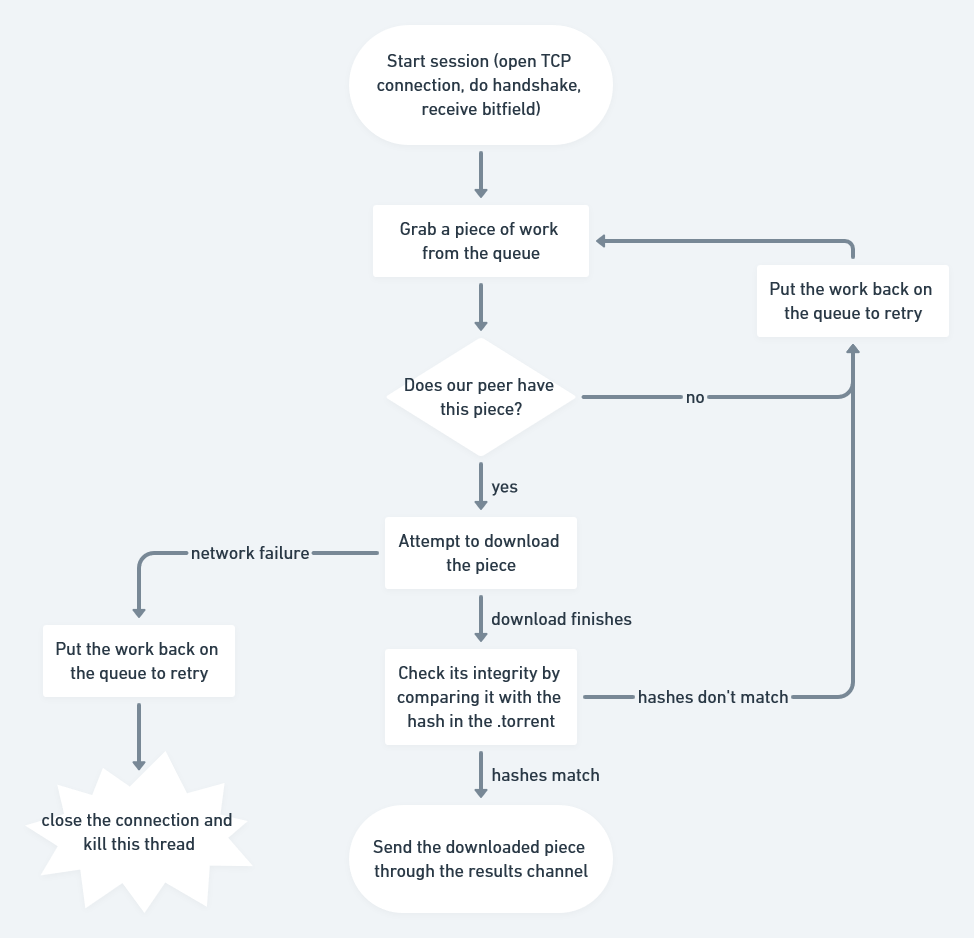
\includegraphics[width=3in,height=3in]{bt_queue.png}
\end{block}
\end{frame}

\begin{frame}
\frametitle{Our Implementation}
\begin{block}{How did we decide to go about implementing a p2p protocol?}
\begin{itemize}
\item Due to time constraints, a full BT client implementation was not acheivable
\item Instead, a far simpler to implement but functionally similar protocol was devised
\item This sharing program is written in go
\end{itemize}
\end{block}
\end{frame}

\begin{frame}
\frametitle{Implementation}
\begin{block}{Core components of our protocol}
\begin{itemize}
\item Centralized metadata "tracker" tracking peers with file
\item Files distributed via message passing algorithm
\item HTTP used for client to tracker communication
\item Metadata serialized via JSON instead of Bencode (better library support)
\item Stripped down messages and passing algorithm
\item Only supports one file at a time
\end{itemize}
\end{block}
\end{frame}

\begin{frame}
\frametitle{Thank you for watching!}
\end{frame}
\end{document}